\section{问题重述}

\subsection{问题背景}

插入表格:
\begin{table}[H]
    \centering
    \begin{tabular}{|p{1.8cm}|p{4.5cm}|p{4.5cm}|p{4.5cm}|}
        \hline
         & 参赛队员 1 & 参赛队员 1 & 参赛队员 1\\\hline
        \textbf{姓名} & & & \\\hline
        \textbf{学号} & & & \\\hline
        \textbf{院系} & & & \\\hline
        \textbf{专业} & & & \\\hline
        \textbf{手机} & & & \\\hline
        \textbf{Email} & & & \\\hline
    \end{tabular} 
    \caption{表格标题}\label{tab-1}
\end{table}

三线表:
\begin{table}[H]
    \centering
    \newcolumntype{F}{>{$}c<{$}}
    \begin{tabular}{FlF}
        \toprule  
         & \text{参数名称} & \text{参数取值}\\
        \midrule
        M & \text{小车质量} & \\
		m & \text{摆杆质量} & \\
		b & \text{小车摩擦系数} & \\
		l & \text{摆杆转动轴心到杆质心的长度} & \\
		I & \text{摆杆惯量} & \\
		F & \text{加在小车上的力} & \\
		x & \text{小车位置} & \\
		\phi & \text{摆杆与垂直向上方向的夹角} & \\
		\theta & \text{摆杆与垂直向下方向的夹角} & \\
        \bottomrule
    \end{tabular}
    \caption{各物理参数}\label{tab-arg}
\end{table}

插入图片,尽量使用H默认不浮动,图片引用使用ref指令,如图\ref{model}所示:
\begin{figure}[H]
	\centering
	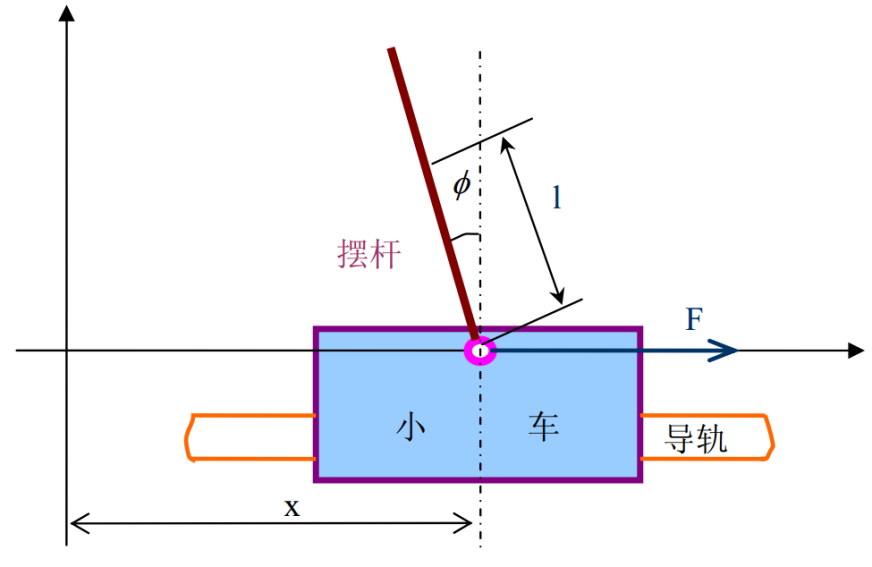
\includegraphics[width=0.6\textwidth]{model}\\
	\caption{简化模型}\label{model}
\end{figure}

插入双栏图片:图片名+图片标题+图片标签,如图\ref{step},\ref{sin}所示:
\dpicl{model}{阶跃干扰信号}{step}{model}{正弦干扰信号}{sin}

\subsection{问题提出}

